%\documentclass[10pt]{article}
%\usepackage[utf8]{inputenc}
%\usepackage[T1]{fontenc}
%\usepackage{amsfonts}
%\usepackage{amssymb}
%\usepackage{geometry}
%\usepackage{pstricks,pst-eucl}
%\usepackage{tikz}
%\usepackage{graphics}
%\usepackage{pslatex}
%\usepackage{lscape}
%\usepackage{eurosym}
%\usepackage{skak}
%\usepackage{chessboard}

\documentclass[12pt, a4paper]{report}
%\documentclass[11pt, a4paper]{article}

%====================== PACKAGES ======================

\usepackage[french]{babel}
\frenchbsetup{StandardLists=true}
\usepackage{enumitem}
\usepackage{pifont}
\usepackage[utf8x]{inputenc}
\usepackage[T1]{fontenc}
%pour gérer les positionnement d'images
\usepackage{float}
\usepackage{amsmath}
\DeclareMathOperator{\dt}{dt}
\usepackage{graphicx}
\usepackage{tabularx}
\usepackage[colorinlistoftodos]{todonotes}
\usepackage{url}
%pour les informations sur un document compilé en PDF et les liens externes / internes
\usepackage[pdfborder=0]{hyperref}
\hypersetup{
	colorlinks = true
	}
%pour la mise en page des tableaux
\usepackage{array}
\usepackage{tabularx}
\usepackage{multirow}
\usepackage{multicol}
\setlength{\columnsep}{50pt}
%espacement entre les lignes
\usepackage{setspace}
%modifier la mise en page de l'abstract
\usepackage{abstract}
%police et mise en page (marges) du document
\usepackage[T1]{fontenc}
\usepackage[top=2cm, bottom=2cm, left=2cm, right=2cm]{geometry}
%Pour les galerie d'images
\usepackage{subfig}

\usepackage{pdfpages}
%\usepackage{tikz}

\usepackage{appendix}

\usepackage{comment}

\usepackage{skak}
\usepackage{chessboard}
%\usepackage{indentfirst}
%\usetikzlibrary{angles, quotes}
%\usetikzlibrary{decorations.pathmorphing}
%====================== INFORMATION ET REGLES ======================
\frenchbsetup{StandardLists=false}
%rajouter les numérotation pour les \paragraphe et \subparagraphe
\setcounter{secnumdepth}{4}
\setcounter{tocdepth}{4}

\hypersetup{							% Information sur le document
pdfauthor = {Stephan Runigo},			% Auteurs
pdftitle = {Recueil d'échec},			% Titre du document
pdfsubject = {Stratégie et tactique du jeu d'échec},		% Sujet
pdfkeywords = {jeu d'échec, stratégie, tactique},	% Mots-clefs
pdfstartview={FitH}}	% ajuste la page à la largeur de l'écran
%pdfcreator = {MikTeX},% Logiciel qui a crée le document
%pdfproducer = {} % Société avec produit le logiciel
%======================== DEBUT DU DOCUMENT ========================
%
\begin{document}
%
%régler l'espacement entre les lignes
\newcommand{\HRule}{\rule{\linewidth}{0.5mm}}
%
%présentation	%
%
%
\begin{titlepage}
%
~\\[1cm]

\begin{center}
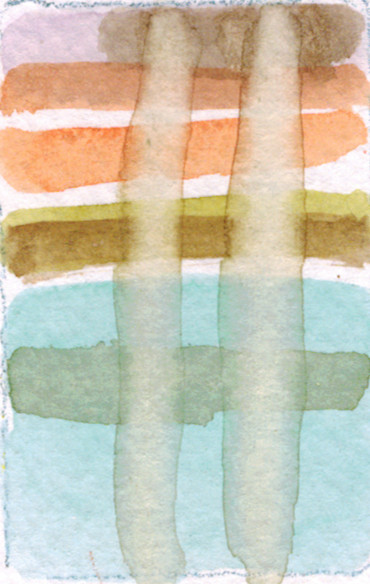
\includegraphics[scale=2]{./presentation/champ06}
\end{center}

\textsc{\Large }\\[0.5cm]

% Title \\[0.4cm]
\HRule

\begin{center}
{\huge \bfseries  Principes élémentaires\\
du jeu d'échec\\[0.4cm] }
\end{center}

\HRule \\[1.5cm]

\begin{center}
%\includegraphics[scale=0.3]{./presentation/ptoleme}
\end{center}

\begin{center}
%\includegraphics[scale=0.3]{./presentation/diagrammesInteractions}
\end{center}


% Author and supervisor
\begin{minipage}{0.4\textwidth}
\begin{flushleft} \large
\emph{Auteur:}\\
Stephan \textsc{Runigo}
\end{flushleft}
\end{minipage}
\begin{minipage}{0.4\textwidth}
\begin{flushright} \large
\emph{Illustration:}\\
Krikri
\end{flushright}
\end{minipage}

\vfill

% Bottom of the page
{\large \today}

\end{titlepage}

\newpage
\begin{center}
\Large
Résumé
\normalsize
\end{center}
\vspace{3cm}
\begin{itemize}[leftmargin=1cm, label=\ding{32}, itemsep=21pt]
\item {\bf Objet : Les ouvertures} .
\item {\bf Contenu : Principes élémentaires} .
\item {\bf Public concerné : Débutant} .
\end{itemize}

\vspace{3cm}



\vspace{3cm}


%

%
%\newpage
%~
%ne pas numéroter cette page
%\thispagestyle{empty}
	%\newpage

\tableofcontents
\thispagestyle{empty}
\setcounter{page}{0}
%ne pas numéroter le sommaire
%
%\newpage
%
%espacement entre les lignes d'un tableau
\renewcommand{\arraystretch}{1.5}
%
%====================== INCLUSION DES PARTIES ======================
%
~
\thispagestyle{empty}
%recommencer la numérotation des pages à "1"
\setcounter{page}{0}
\newpage
%	%
\chapter{Problème de stratégie}
%

\newpage

\section{Énoncé des exercices}

Dans les problèmes suivant, l'analyse de la position permet de trouver un bon coup stratégique.

\subsection{Exercice 25}%%%%%%%%%%%%%%%%%%%%%%%%%%%%%%%%%%%%%%%%%%%%

\newgame
\fenboard{r4rk1/2p3b1/3p3p/p1pPp1p1/2P5/5PN1/PP4PP/1R3RK1 b − − 0 1}
\storegame{strategie25}
\begin{minipage}{0.45\textwidth}
\hspace{0.7cm}Il y a un bon coup stratégique pour les noirs.
\vspace{0.5cm}

\end{minipage}
\hfill
\begin{minipage}{0.45\textwidth}
\chessboard[
%showmover=false,
inverse,markstyle=leftborder,
]%\showboard
\end{minipage}

\subsection{Exercices 28} %%%%%%%%%%%%%%%%%%%%%%%%%%%%%%%%%%%%%%%%%%%%
\subsubsection{Exercice a} %%%%%%%%%%%%%%%%%%%%%%%%%%%%%%%%%%%%%%%%%%%%

\newgame
\fenboard{rnbqk2r/pp3ppp/2p2n2/3p2B1/1b1P4/2NB1Q2/PPP2PPP/R3K1NR b − − 0 1}
\storegame{strategie28a}
\begin{minipage}{0.45\textwidth}
\hspace{0.7cm} Ici, il y a plusieurs bon coup pour les noirs.
\vspace{0.5cm}

\hspace{0.7cm} Que joueriez-vous ?
\vspace{0.5cm}

\hspace{0.7cm} Quelle est la menace stratégique des blancs ? % Comment l'empêcher ?
\vspace{0.5cm}

\end{minipage}
\hfill
\begin{minipage}{0.45\textwidth}
\chessboard[
%showmover=false,
inverse,markstyle=leftborder,
]%\showboard
\end{minipage}

%\item 28b %%%%%%%%%%%%%%%%%%%%%%%%%%%%%%%%%%%%%%%%%%%%\subsection{28b}
\subsubsection{Exercice b} %%%%%%%%%%%%%%%%%%%%%%%%%%%%%%%%%%%%%%%%%%%%

\newgame
\fenboard{rn2k2r/pp3p2/2p1bp1p/3p4/1b1P4/P1NB1N2/1PP2PPP/R3K2R b − − 0 1}
\storegame{strategie28b}
\begin{minipage}{0.45\textwidth}
\hspace{0.7cm} Les noirs peuvent, soit échanger leur fou avec le cavalier, soit conserver leur fou.
\vspace{0.5cm}

\hspace{0.7cm} Quel est le meilleur choix ?
\vspace{0.5cm}

\end{minipage}
\hfill
\begin{minipage}{0.45\textwidth}
\chessboard[
%showmover=false,
inverse,markstyle=leftborder,
]%\showboard
\end{minipage}


%\item 28c %%%%%%%%%%%%%%%%%%%%%%%%%%%%%%%%%%%%%%%%%%%%\subsection{28c}
\subsubsection{Exercice c} %%%%%%%%%%%%%%%%%%%%%%%%%%%%%%%%%%%%%%%%%%%%

\newgame
\fenboard{r3k2r/pp1n1p2/2p1bp1p/3p4/3P4/P1PB1N2/2P2PPP/R3K2R b − − 0 1}
\storegame{strategie28c}
\begin{minipage}{0.45\textwidth}
\hspace{0.7cm}Ici, il y a un coup difficile à trouver pour les blancs. C'est un coup avec des idées, un plan.
\vspace{0.5cm}

\hspace{0.7cm} Ou se trouve la faiblesse des noirs ? Ou se trouve la faiblesse des blancs ? 
\vspace{0.5cm}

\hspace{0.7cm} Comment attaquer ces faiblesses ? Comment les défendre ? 
\vspace{0.5cm}

\end{minipage}
\hfill
\begin{minipage}{0.45\textwidth}
\chessboard
\end{minipage}

%\item 33 %%%%%%%%%%%%%%%%%%%%%%%%%%%%%%%%%%%%%%%%%%%%%%%%\subsection{33}
\subsection{Exercice 33} %%%%%%%%%%%%%%%%%%%%%%%%%%%%%%%%%%%%%%%%%%%%

\newgame
\fenboard{rn1qk2r/ppp1ppbp/3p2pn/8/2PP4/2N2P2/PP2BPPP/R1BQK2R w − − 0 1}
\storegame{strategie33}
\begin{minipage}{0.45\textwidth}
\hspace{0.7cm} Les noirs viennent de sortir leur cavalier. Quel est leur plan ?
\vspace{0.5cm}

\hspace{0.7cm} Les blancs jouent un coup qui stope le plan des noirs.
\vspace{0.5cm}

\end{minipage}
\hfill
\begin{minipage}{0.45\textwidth}
\chessboard[pgfstyle=color,
opacity=0.3,
color=green,
markfield=g8,
markfield=h6,
]
\end{minipage}
%\end{itemize}
%%%%%%%%%%%%%%%%%%%%%%%%%%%%%%%%%%%%%%%%%%%%%%%%%%%%%%%%%
%\begin{itemize}[leftmargin=0.7cm, itemsep=0pt]
%\item  \end{itemize}

%
%
%

%
%
\begin{appendix}
%

%%%%%%%%%%%%%%%%%%%%%
\chapter{Le matériel}
%%%%%%%%%%%%%%%%%%%%%


La valeur conventionnelle des pièces permet de détecter les échanges favorable.

%\multicolumn{4}{|c|}{}\\%\cline{2-7}\hline
\begin{center}
\begin{tabular}{ccc}
Pièce & valeur & cas particulier \\
Pion & 3 temps & Plus fort au centre \\
Cavalier & 3 pions & Plus fort dans les positions fermé \\
Fou & 3 pions & Plus fort dans les positions ouvertes\\
Tour & 5 pions & Forte sur les colonnes ouvertes \\
Dame & 9 pions & Plus forte en attaque qu'en défense\\
%roi &  & \\
\end{tabular}
\end{center}


%\begin{itemize}[leftmargin=1cm, label=\ding{32}, itemsep=1pt]
%\item {\bf } : \end{itemize}

%%%%%%%%%%%%%%%%%%%%%%%%%%%%%%%%%%%%%%%%%%%%%%%%%%%%%%%

%
\newpage
%

%%%%%%%%%%%%%%%%%%%%%
\chapter{L'espace}
%%%%%%%%%%%%%%%%%%%%%

%%%%%%%%%%%%%%%%%%%%%
\section{Espace contrôlé}
%%%%%%%%%%%%%%%%%%%%%

%C'est les cases accessible par les pièces (pas par les pions)

Lors de 

\begin{minipage}{0.4\textwidth}

\begin{center}
\newgame
\mainline{1. e4 }

\chessboard[color=red,
	markstyle=color,markfields=a6,
	markfields=e2,markfields=d3,markfields=c4,markfields=b5,
	markfields=f3,markfields=g4,markfields=h5,]
\end{center}
L'ouverture du pion roi offre 8 cases.
\end{minipage}
\begin{minipage}{0.5\textwidth}
\begin{center}
\newgame
\mainline{1. d4 }

\chessboard[color=red,
	markstyle=color,markfields=h6,
	markfields=d2,markfields=e3,markfields=f4,markfields=g5,
	markfields=d3,]
\end{center}
L'ouverture du pion roi offre 6 cases.
\end{minipage}

\begin{minipage}{0.4\textwidth}
\begin{center}
\newgame
\mainline{1. c4 }

\chessboard[color=red,
	markstyle=color,markfields=d4,
	markstyle=color,markfields=e5,]
\end{center}
Le cavalier f3 contrôle les deux cases centrales d4 et e5.
\end{minipage}
\begin{minipage}{0.4\textwidth}
\begin{center}
\newgame
\mainline{1. Nf3 }

\chessboard[color=red,
	markstyle=color,markfields=d4,
	markstyle=color,markfields=e5,]
\end{center}
Le cavalier f3 contrôle les deux cases centrales d4 et e5.
\end{minipage}

\newgame

\mainline{1. e4 e5 2. Nf3 Nc6}

\begin{center}
\chessboard
\end{center}

%\newchessgame
\newgame

\def\empharea{ h8-f4 }
\chessboard[emphstyle=\color{red},
empharea=\empharea]


%%%%%%%%%%%%%%%%%%%%%
%\section{Le temps}
%%%%%%%%%%%%%%%%%%%%%

\fenboard{r5k1/1b1p1ppp/p7/1p1Q4/2p1r3/PP4Pq/BBP2b1P/R4R1K w − − 0 20}
\mbox{}
\bigskip
\showboard
\mainline{20.Qxb7 Rae8 21.Qd5}





%\newgame
%\mainline{1. Nf3 }
%\def\empharea{ f3-f3 }
%\chessboard[color=red,
%	markstyle=color,markfields=d4,
%	markstyle=color,markfields=e5,
%	emphstyle=\color{green},
%	empharea=\empharea]
%%%%%%%%%%%%%%%%%%%%%%%%%%%%%%%%%%%%%%%%%%%%%%%%%%%%%%%

%
\newpage
%

%%%%%%%%%%%%%%%%%%%%%
\chapter{Le temps}
%%%%%%%%%%%%%%%%%%%%%

%%%%%%%%%%%%%%%%%%%%%
%\section{L'espace}
%%%%%%%%%%%%%%%%%%%%%

C'est les cases accessible par les pièces (pas par les pions)

e4 offre 8 cases, e5 offre 6 cases.


C'est le nombres de mouvement de pièces pour atteindre la position.

%\begin{itemize}[leftmargin=1cm, label=\ding{32}, itemsep=1pt]
%\item {\bf } : \end{itemize}




\fenboard{r5k1/1b1p1ppp/p7/1p1Q4/2p1r3/PP4Pq/BBP2b1P/R4R1K w − − 0 20}

\mbox{}
\bigskip

\showboard


\mainline{20.Qxb7 Rae8 21.Qd5}







%%%%%%%%%%%%%%%%%%%%%%%%%%%%%%%%%%%%%%%%%%%%%%%%%%%%%%%

%
\newpage
%
%\input{./annexe/.tex}
%
\newpage
%
\end{appendix}
%

%
%====================== INCLUSION DE LA BIBLIOGRAPHIE ======================
%
%récupérer les citation avec "/footnotemark"
%\nocite{*}
%choix du style de la biblio
\bibliographystyle{plain}
%inclusion de la biblio
\cleardoublepage
\addcontentsline{toc}{chapter}{Bibliographie}
\bibliography{bibliographie.bib}
%\newpage
%\input{./glossaire/glossaire.tex}
%\newpage
%\input{./annexes/annexes.tex}
\end{document}
%%%%%%%%%%%%%%%%%%%%%%%%%%%%%%%%%%%%%%%%%%%%%%%%%%%%%%%%%%%%%%%%%%%%%%%%%%%%%%%%%
